\documentclass[11pt,a4paper]{article}
\usepackage[margin=25mm]{geometry}
\usepackage[T1]{fontenc}
\usepackage{lmodern,microtype,amsmath,amssymb,amsthm,graphicx,booktabs,tabularx,xcolor,listings,fancyhdr}
\usepackage{xurl,placeins}
\usepackage[hidelinks]{hyperref}
\hypersetup{pdftitle={StopLane: Measuring and Removing Cancellation Bottlenecks in PHP Streaming Gateways},pdfauthor={Shivam Gupta}}
\usepackage[font=small,labelfont=bf]{caption}
\definecolor{ink}{HTML}{24516B}
\lstset{basicstyle=\ttfamily\footnotesize,breaklines=true,frame=single,rulecolor=\color{ink},columns=fullflexible,keepspaces=true,showstringspaces=false}
\newtheorem{proposition}{Proposition}
\pagestyle{fancy}\fancyhf{}\fancyhead[L]{\small Gupta | StopLane}\fancyhead[R]{\small Research manuscript}\fancyfoot[C]{\thepage}
\setlength{\headheight}{14pt}
\setlength{\parskip}{4pt}\setlength{\parindent}{0pt}
\newcommand{\GoodGateway}{11.9}
\newcommand{\GoodGatewayMax}{15.9}
\newcommand{\GoodProvider}{22.1}
\newcommand{\GoodAdmission}{2.4}
\newcommand{\BaselineGateway}{1269.3}
\newcommand{\CallbackGateway}{770.4}
\newcommand{\UncoopProvider}{1272.6}
\newcommand{\UncoopGateway}{12.6}
\newcommand{\SavedTicks}{88.8}

\title{\textbf{StopLane: Measuring and Removing Cancellation Bottlenecks in PHP Streaming Gateways}}
\author{Shivam Gupta\\\small Independent Researcher, India and United Arab Emirates\\\small\href{mailto:shivam1720406@gmail.com}{shivam1720406@gmail.com}}
\date{14 October 2026}
\begin{document}
\maketitle
\begin{abstract}
A streaming application can accept a user's intention to stop while its gateway continues waiting for, or forwarding, an upstream response. We study cancellation in a PHP deployment where three independently familiar mechanisms interact: native session locking, finite PHP-FPM capacity, and cancellation checks tied to arriving response chunks. StopLane combines a three-stage diagnostic contract with an authenticated reference gateway and a reproducible failure-injection benchmark. A locally frozen factorial protocol executes 320 trials through nginx, PHP-FPM and a controlled HTTP provider; 60 additional trials vary polling and upstream cooperation. Under a saturated pool and a 900 ms upstream silence, early session release, reserved control capacity and timed polling jointly reduce median request-to-gateway-end latency from \BaselineGateway\ ms to \GoodGateway\ ms. Removing either release or reservation prevents observed cancellation before natural completion in the corresponding saturated tests. Callback-only observation instead takes \CallbackGateway\ ms. A noncooperative provider continues for \UncoopProvider\ ms despite gateway termination in \UncoopGateway\ ms. A separate pinned Symfony comparison tests an existing library implementation of timed observation. The contribution is an end-to-end PHP cancellation benchmark and a deployment contract that distinguishes control admission, gateway termination and upstream work termination. It does not establish model-quality improvements, production latency guarantees or token-billing savings.
\end{abstract}
\textbf{Keywords:} PHP-FPM; streaming gateways; cancellation; session locks; bulkhead isolation; reproducible systems evaluation.

\section{Introduction}
A PHP application that streams an external service occupies several resources simultaneously: an HTTP connection, a PHP-FPM worker, possibly a session lock, and an upstream request. A stop button often closes the browser's stream or sends a separate cancellation request. The latter has an appealing interpretation: the gateway records the instruction, notices it and closes its upstream transport. However, the cancellation request must itself be scheduled and authenticated. Its path may depend on exactly the resources held by the stream it needs to stop.

Consider a gateway with three FPM workers. Three ongoing streams occupy all three workers. A fourth HTTP request, intended to cancel one stream, queues until a worker becomes available. Releasing the stream's session lock does not create a worker. Reserving a control worker avoids that queue, but does not help if the cancellation handler must acquire a native session lock retained by the target stream. Removing both dependencies still leaves a third issue: a gateway that checks its cancellation marker only inside a body callback receives no observation opportunity during a silent upstream period.

These are documented mechanisms, not newly discovered PHP defects. The PHP manual describes native session serialization and early session closure \cite{phpsession}; FPM documents the concurrency cap \cite{fpm}; and isolation is the established bulkhead pattern \cite{bulkhead}. The engineering question is their composition: \emph{which observable evidence demonstrates that a deployed stop path remains effective under the same load and silence that make a long-running stream expensive?}

We address this question with StopLane, a name for a reference deployment and audit rather than a new networking primitive. The artifact provides explicit cancellation requests, ownership checks, generation-specific monotone markers, and independent polling opportunities. A full factorial experiment removes each deployment ingredient and observes actual HTTP, FPM and upstream lifecycles. The aim is to expose a misleading success criterion: a successful HTTP cancellation response establishes neither timely observation by the gateway nor termination of provider work.

The study contributes (1) a staged cancellation contract and conditional latency decomposition; (2) an executable PHP reference and capacity-matched dispatch configurations; (3) a randomized factorial benchmark with complete machine-readable traces, independent consistency checks and a library comparison; and (4) a deployment procedure that makes the performance cost of reserving control capacity explicit. The intended applications include chat interfaces, long-running report generation, retrieval pipelines and tool-oriented gateways. These applications motivate the experiment; their adoption and commercial value are not estimated here.

\section{Prior work and contribution boundary}
\subsection{PHP sessions, dispatch capacity and streaming}
Native PHP session data is ordinarily serialized by a lock; \texttt{session\_write\_close()} persists changes and ends the active session \cite{phpsession}. Retaining that lock during remote I/O serializes requests from the same session. PHP-FPM's \texttt{pm.max\_children} independently limits simultaneous requests \cite{fpm}. These dependencies occur before the cancellation marker is published, whereas the gateway's polling behavior occurs afterwards.

PHP connection handling is another distinct mechanism. The manual describes detection when the script attempts output \cite{phpconnection}; this makes a browser disconnect different from a separate authenticated cancellation request. nginx buffering and client-abort handling can also affect what reaches the FastCGI application \cite{nginx}. Our primary tests deliberately keep the browser-side stream open and disable FastCGI buffering. They isolate explicit stop requests rather than comparing proxy disconnect-detection settings.

The use of a timer while awaiting network progress is established. libcurl's multi interface allows application-controlled event-loop progression \cite{curlmulti}; PHP exposes a selectable wait with a timeout \cite{phpselect}. Symfony HttpClient supplies streamed timeout chunks and explicit response cancellation \cite{symfony}. Amp supplies cooperative cancellation abstractions \cite{amp}. The proposed contract can be implemented using these existing libraries; the direct cURL implementation is a small observable reference, not a claim that applications require a new HTTP client.

Laravel warrants particular care: its documented default permits concurrent same-session requests, and route-level blocking is optional \cite{laravel}. Consequently, our native-file-session result must not be generalized to all Laravel applications, even those using Laravel's file session driver. A framework integration must inspect its actual middleware and lock lifecycle.

\subsection{Inference cancellation and workload recovery}
Inference servers already recognize cancellation as a resource-management concern. Triton's documentation describes explicit request cancellation and backend checks \cite{triton}; vLLM exposes abort operations \cite{vllm}. These interfaces make upstream cooperation an explicit condition, rather than a consequence that a gateway can infer merely from closing its socket. PipeInfer studies early cancellation of invalidated speculative inference \cite{pipeinfer}; that is a different locus of cancellation from admission of an application's control request.

De Souza's public request-cancellation benchmark compares polling and push mechanisms, work waste, KV residency and survivor latency through a discrete-event simulation \cite{desouza}. It is close in motivation. Our experiment instead executes a real PHP web stack and measures the control request before its cancellation signal becomes available to a polling strategy. We do not use the simulation's performance numbers as production evidence, and do not claim new discovery of polling delay or delayed resource reclamation.

\begin{table}[t]
\centering\small
\begin{tabularx}{\linewidth}{@{}p{0.25\linewidth}XX@{}}
\toprule
Existing mechanism & Established capability & Question tested here\\\midrule
Native session closure & End session serialization & Can cancellation acquire its session promptly?\\
FPM worker pools; bulkheads & Partition concurrency & Is control admitted while data workers are occupied?\\
Symfony; libcurl; Amp & Timed I/O and cooperative cancellation & Are checks reached during body silence?\\
Inference-server abort APIs & Request provider termination & Does provider work actually end after local teardown?\\
Cancellation simulation & Model post-cancel resource recovery & What delay precedes signal publication in a PHP stack?\\\bottomrule
\end{tabularx}
\caption{Positioning against existing tools and research. Each row credits an existing capability; the study evaluates the deployment boundary connecting them.}
\label{tab:prior}
\end{table}

\subsection{Novelty assessment}
The literature search covered PHP session locking, FPM pool saturation, streaming cancellation, cancellation benchmarks, library timeout APIs and inference-server abort behavior. Primary documentation and the closely related public benchmark were inspected. The reviewed sources establish the individual techniques; they did not supply the exact capacity-matched PHP factorial experiment reported here. This is a bounded novelty claim about the artifact and evidence. A search cannot establish that nobody has previously composed these techniques, and naming the artifact does not establish patentability.

\section{A staged cancellation contract}
\subsection{Events and outcomes}
For a target generation $g$, let $t_0$ be the client timestamp immediately before issuing its explicit stop request. Let $t_p$ denote publication of a cancellation marker after dispatch and authentication; $t_o$ the gateway's first observation of that marker; $t_g$ gateway termination; and $t_u$ upstream work termination. Gateway observation may never occur before natural completion; in that case $t_o$ is absent and the run is recorded as an unsuccessful cancellation, even if the control request eventually returns successfully.

We report three different latencies:
\begin{equation}
L_p=t_p-t_0,\qquad L_g=t_g-t_0,\qquad L_u=t_u-t_0.
\end{equation}
An HTTP acknowledgement follows publication but is not a gateway-termination acknowledgement. Natural completion can yield $t_g<t_p$. Conversely, an uncooperative upstream can yield $t_g\ll t_u$. Both orders are valid observations rather than missing or failed measurements.

\begin{figure}[t]
\centering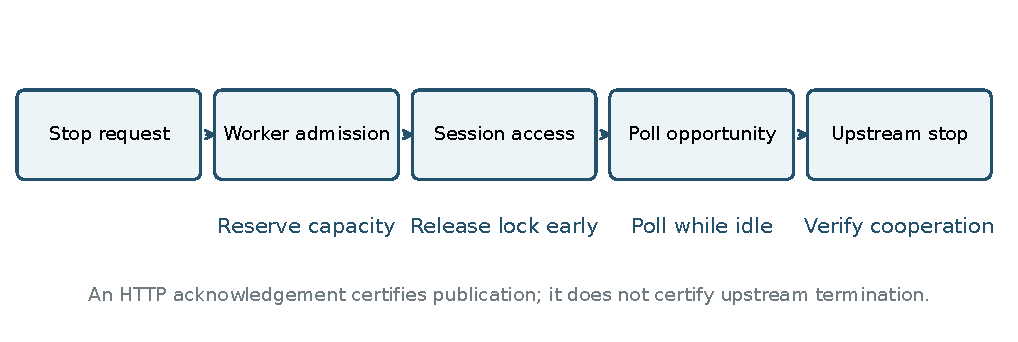
\includegraphics[width=\linewidth]{../figures/architecture.pdf}
\caption{The control path crosses admission, authentication and observation boundaries before upstream termination. Reservation, lock release and idle polling address different dependencies.}
\label{fig:architecture}
\end{figure}

\subsection{Conditional latency bound}
Define $A$ as an upper bound on control dispatch, including network and worker waiting; $S$ as an upper bound on authentication-related lock waiting and processing; $W$ as a bound on marker publication and visibility; $P$ as a bound on the time to the next cancellation check; $G$ as a bound on local transport teardown; and $U$ as an upstream reaction bound after that teardown. These are wall-clock bounds on the deployed mechanisms, not configuration values alone.

\begin{proposition}[Staged termination bound]
If a cancellation request targets an active generation, marker publication succeeds, and the six bounds above hold, then
\begin{equation}
L_g\leq A+S+W+P+G,\qquad
L_u\leq A+S+W+P+G+U.
\label{eq:bound}
\end{equation}
\end{proposition}
\begin{proof}
Dispatch and authentication complete by $t_0+A+S$. Publication becomes visible within a further $W$. The next check observes the monotone marker within $P$, and local teardown completes within $G$. Upstream cooperation supplies the final $U$. Adding the bounds yields the two inequalities. Natural completion before these deadlines can only shorten termination latency; it does not establish observation of cancellation.
\end{proof}
This elementary decomposition is a diagnostic specialization of bounded cooperative cancellation, not a new scheduling theorem. Its value is identifying which assumption a measurement must test. A 20 ms \texttt{curl\_multi\_select} argument alone does not prove $P\leq20$ ms: blocking callbacks, DNS behavior, scheduling pauses or blocking marker storage can enlarge the interval between checks.

\begin{proposition}[Obstructions in the tested deployment family]
Suppose cancellation is served by the same finite FPM pool as streams, all workers are occupied, and no occupied request releases a worker before residual time $R$. Then publication cannot begin before $t_0+R$. If the cancel handler instead has a free worker but must acquire a session lock retained by the target until time $t_\ell$, it cannot publish before $t_\ell$. Finally, if observation occurs only on body callbacks and no callback occurs during an interval of length $H$ following publication, observation cannot occur during that interval.
\end{proposition}
\begin{proof}
A queued request cannot execute its publication instruction before an FPM worker is assigned. A blocking session acquisition cannot advance to publication before lock release. A callback-only marker check cannot run in an interval containing no callback. Each lower bound follows from its corresponding execution dependency.
\end{proof}
The restrictions matter. A stateless authenticated control route can remove the session dependency without early session release. An asynchronous execution system can remove the shared FPM dispatch dependency without a dedicated pool. These are alternative implementations of the contract, not counterexamples to the propositions.

\section{Reference implementation}
\subsection{Authenticated, generation-specific cancellation}
The PHP reference creates a server-side random actor identifier and CSRF token during session initialization. A stream request must present the session cookie and matching token. Each generation has a distinct 128-bit identifier and an immutable owner record. Cancellation uses POST, verifies the same CSRF token and compares the recorded owner with the authenticated actor. A cross-session request cannot cancel a generation merely by knowing its identifier.

The marker is an immutable file created with exclusive-create semantics. Repeated cancellation is idempotent. IDs are never reused: a late cancellation for one generation cannot affect another, and an attempted duplicate stream ID returns a conflict. Marker existence, rather than marker contents, is the cancellation signal. This permits atomic publication at creation; \texttt{clearstatcache()} avoids stale PHP stat-cache decisions. Records live in a private single-host test directory. A distributed deployment would need equivalent monotonicity, scope, visibility and retention guarantees from its state store.

The gateway copies authentication values before optionally closing the active session. It does not mutate session state after that closure. The cancellation handler closes its own session promptly after authentication and before publishing. This limits control-path lock occupancy but cannot undo a lock still held by the target.

\subsection{Dispatch isolation and observation}
The shared route sends streams and cancellation to three general-purpose workers. The isolated route sends streams to two workers and cancellation to one control worker. Each route thus has three dispatch workers. Reserving one worker reduces immediate stream capacity from three to two; an experiment that added a fourth worker would confound isolation with additional capacity.

The direct timed implementation progresses the cURL multi handle, checks a marker between waits, and uses a configurable bounded wait. A body callback also checks the marker before forwarding bytes. The callback-only ablation uses blocking \texttt{curl\_exec()} and checks solely when body data arrives. Once cancellation is observed, the multi implementation removes the handle and drops the local handle reference; the callback implementation returns zero to abort the transfer. The trace records which path observed the marker.

\begin{lstlisting}[float=t,language=PHP,caption={Core timed-observation pattern; the complete authenticated implementation is in the artifact.}]
while (true) {
    clearstatcache(true, $marker);
    if (is_file($marker)) { $cancelled = true; break; }
    do {
        $status = curl_multi_exec($multi, $running);
    } while ($status === CURLM_CALL_MULTI_PERFORM);
    if ($status !== CURLM_OK || !$running) break;
    if (curl_multi_select($multi, $pollSeconds) === -1) {
        usleep((int) ($pollSeconds * 1_000_000));
    }
}
curl_multi_remove_handle($multi, $response);
unset($response);
\end{lstlisting}

The reference intentionally separates explicit stop requests from browser transport closure: \texttt{ignore\_user\_abort(true)} keeps lifecycle logging reachable, and the client retains its stream connection during the tests. nginx FastCGI buffering is disabled. The benchmark does not claim to implement every browser-disconnect path or to certify provider billing behavior.

\section{Experimental method}
\subsection{Frozen design and actual execution}
The main protocol was locally frozen at Git commit \texttt{b685e41}, after exploratory pilot runs and before primary collection. It specifies the complete $2\times2\times2\times2\times2$ factorial: session release, reserved control capacity, timer polling, two versus three offered streams, and regular versus silent upstream output. Ten randomized blocks each contain all 32 cells, for 320 primary trials. Randomization uses seed 1720406. The artifact retains all primary runs; pilot measurements do not enter primary tables.

Each trial starts its target before the filler streams. Readiness barriers wait for the expected number of active upstream requests: two in the isolated route under three offered streams, and three in the corresponding shared route. The stop request is issued 120 ms after that barrier. Each stream uses a distinct session; the cancel request uses the target's session. The isolated route's third offered stream queues until a data worker is available. Trial completion waits for every offered stream and its upstream workload, preventing overlap between trials.

The provider is a controlled HTTP/SSE service, not an inference simulator. It executes a 1.4-second loop with approximately 10 ms work opportunities. Regular output emits roughly every 20 ms; silent output emits no body data during its first 900 ms. These timings exercise network and callback conditions without requiring a particular language model to produce them. Loop iterations are called \emph{synthetic work ticks}. They are never treated as model tokens, FLOPs, energy or billable operations. Cooperative provider code tests socket closure each loop and stops promptly after observing it.

The actual path is client HTTP $\rightarrow$ nginx $\rightarrow$ FastCGI $\rightarrow$ PHP-FPM $\rightarrow$ HTTP provider. Both route configurations reside as separate idle pools under one master; only one route is exercised in a trial. Thus each comparison has three available dispatch workers, although the harness has six resident children. No resident-memory comparison is made. A single-host test is deliberately small enough for full trace inspection.

\subsection{Measurements, controls and analysis}
PHP records handler entry, session acquisition, upstream opening, marker publication, marker observation and gateway termination. The independently running provider records start, peer closure and work termination. Client timestamps bracket the cancellation HTTP request. All use one host wall clock. The verifier rejects negative reported intervals and channel-local timestamp regressions; adjustment of the host clock remains a validity threat.

The locally specified secondary controls comprise ten noncooperative-upstream runs and fifty timer-wait runs: 5, 10, 20, 50 and 100 ms, ten each. The noncooperative provider detects closure but continues its loop, demonstrating the scope of gateway control. A later protocol extension specifies a pinned Symfony library comparison separately from the primary factorial; it is not pooled into primary estimates.

Every cell is reported with observed cancellations, median publication and termination latencies, and termination range. Selected contrasts pair configurations by randomized block. A 10,000-resample paired bootstrap of the median difference uses seed 20406. These intervals describe repeated execution on this machine; ten repeats cannot establish a production p99 or a distribution-free operational service level. The independent raw-trace verifier imports neither the runner nor the analysis implementation.

\paragraph{Recorded environment.} The main run used PHP 8.4.26  (build: Sep 22 2026 15:00:02) (NTS); nginx/1.31.6; libcurl 8.22.0; Python 3.9.6; and Apple M4 Pro. All measured services ran locally on macOS-27.0.1-arm64-arm-64bit. Exact libcurl features and dependency values are retained in the machine-readable environment file.


\section{Results}
\subsection{The controls solve different bottlenecks}
Table~\ref{tab:ablation} reports the saturated, silent condition. With all three controls disabled, the gateway naturally completes after a median \BaselineGateway\ ms measured from the stop request. Enabling only release does not supply control dispatch capacity; enabling reservation while retaining the target's native session lock does not supply session access. These cases produce a valid eventual cancellation response but no gateway observation before completion. One shared-pool trial publishes its marker 1.8 ms before gateway termination, after the last observation opportunity. The trace still records natural completion; publication order alone would misclassify that race.

Enabling release and reservation admits the marker quickly. However, callback-only polling observes it only when the provider's silent period ends: median gateway termination is \CallbackGateway\ ms. Enabling all three controls brings median marker publication to \GoodAdmission\ ms and gateway termination to \GoodGateway\ ms, with an observed maximum of \GoodGatewayMax\ ms in this ten-run cell. Cooperative provider work ends after median \GoodProvider\ ms.

\begin{table}[t]\centering\small
\begin{tabular}{@{}ccc r r r r@{}}\toprule Release & Reserve & Timer & Observed & Publish & Gateway & Gateway range\\ & & & cancellation & (ms) & (ms) & (ms)\\\midrule
0 & 0 & 0 & 0/10 & 1270.4 & 1269.3 & 1264.3--1276.4 \\
0 & 0 & 1 & 0/10 & 1274.4 & 1273.6 & 1268.1--1278.7 \\
0 & 1 & 0 & 0/10 & 1272.5 & 1271.7 & 1265.4--1277.5 \\
0 & 1 & 1 & 0/10 & 1274.3 & 1273.9 & 1261.3--1277.3 \\
1 & 0 & 0 & 0/10 & 1272.0 & 1271.1 & 1266.0--1278.1 \\
1 & 0 & 1 & 0/10 & 1272.5 & 1271.5 & 1269.0--1276.6 \\
1 & 1 & 0 & 10/10 & 1.5 & 770.4 & 766.8--777.4 \\
1 & 1 & 1 & 10/10 & 2.4 & 11.9 & 9.3--15.9 \\
\bottomrule\end{tabular}

\caption{All eight configurations with three offered streams and silent output; ten trials per row. ``Observed cancellation'' excludes natural completion. Publication after natural gateway termination is possible and retained.}
\label{tab:ablation}\end{table}

\begin{figure}[t]\centering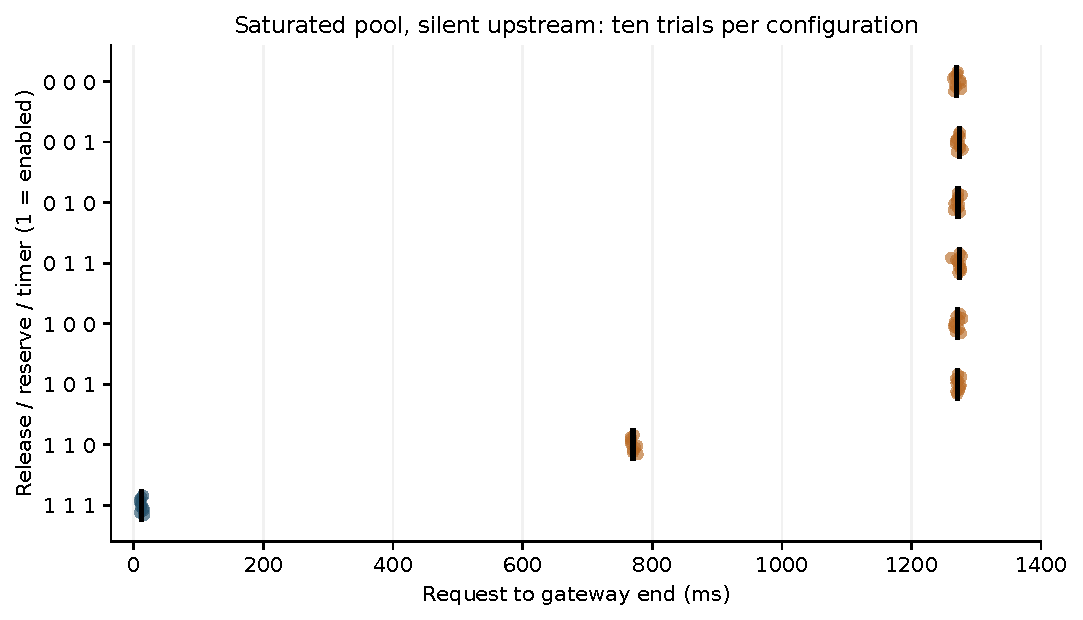
\includegraphics[width=\linewidth]{../figures/ablation.pdf}
\caption{Individual saturated-silent gateway termination measurements. Black marks show medians. The fully enabled configuration terminates promptly; configurations with blocked admission finish naturally. Callback-only observation lies between these outcomes.}
\label{fig:ablation}\end{figure}

The paired median reduction from the fully disabled row to the fully enabled row is 1257.1 ms, with a descriptive paired-bootstrap interval of [1253.7, 1263.4] ms. This contrast combines all three controls; the ablation rows identify the distinct failure boundaries rather than attributing the total reduction to one primitive.


Across the full factorial, the observed cancellation flag agrees in all 320 trials with the deployment-family prediction: the session must be released and either control capacity must be reserved or one shared worker must remain available. Regular output makes callback-only observation reasonably prompt in the admitted cases; silent output exposes its dependence on arriving bytes. The complete cell table in Appendix~\ref{app:cells} preserves both workload conditions rather than averaging away this interaction.

\subsection{Teardown does not imply termination}
The noncooperative control still observes cancellation and terminates its gateway in median \UncoopGateway\ ms, but the provider continues until its ordinary end, median \UncoopProvider\ ms after the request. Figure~\ref{fig:limits} shows this separation directly. The experiment falsifies the inference that a local cancellation flag or successful cURL teardown, without provider evidence, certifies saved upstream computation.

Relative to the fully disabled saturated-silent row, the cooperative fully enabled row reduces median total synthetic work ticks by \SavedTicks\ percent. This is an illustrative reduction in the controlled workload's loop duration. It includes work before the cancellation request and does not measure token billing, GPU occupancy or actual inference cost.

\begin{figure}[t]\centering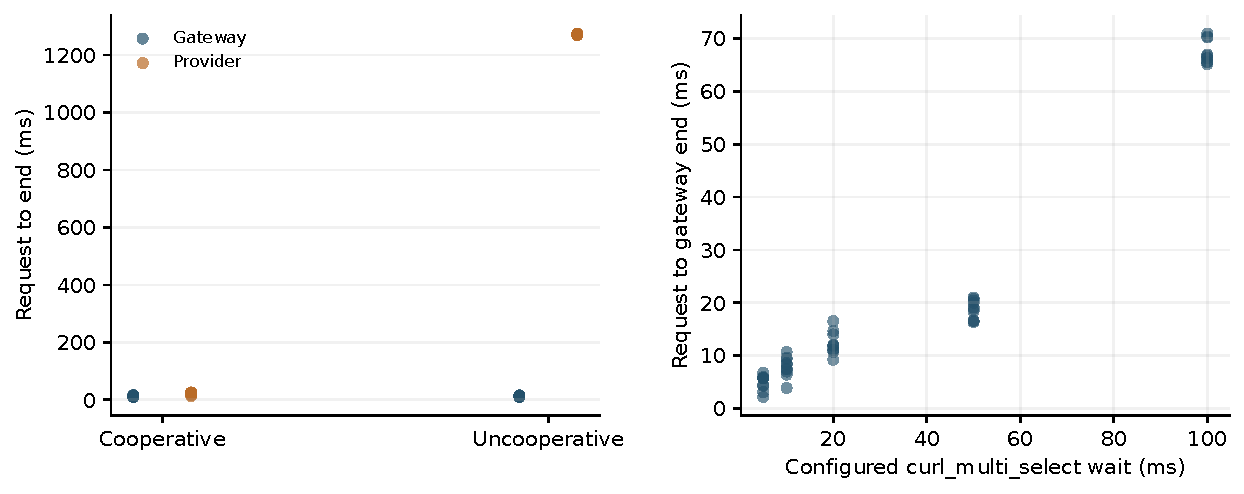
\includegraphics[width=\linewidth]{../figures/limits.pdf}
\caption{Left: individual gateway and provider termination times with all three controls enabled. The provider-cooperation assumption changes upstream termination while preserving rapid gateway termination. Right: configured wait intervals in the timer sweep, with ten observations per interval. Wait settings alone are not hard wall-clock guarantees.}
\label{fig:limits}\end{figure}

\subsection{Existing library comparison and polling tradeoff}
\begin{table}[ht]\centering\small\begin{tabular}{@{}lccrrr@{}}\toprule Client & Release & Reserve & Observed & Gateway (ms) & Range (ms)\\\midrule
symfony & 1 & 1 & 10/10 & 15.5 & 11.0--19.9 \\
symfony & 0 & 1 & 0/10 & 1272.5 & 1268.5--1275.6 \\
symfony & 1 & 0 & 1/10 & 1273.1 & 1264.8--1281.6 \\
curl & 1 & 1 & 10/10 & 11.9 & 10.7--15.0 \\
\bottomrule\end{tabular}\caption{Separate Symfony v8.1.9 extension: three offered streams, silent provider and 20 ms timed observation; ten randomized blocks.}\label{tab:library}\end{table}
Symfony's documented timeout-aware stream and response cancellation satisfy the same observation contract when release and reservation are enabled: 10/10 trials observe cancellation, with median termination 15.5 ms. Without release, no trial records observation. Without reservation, one of ten trials records a late observation after the provider has already ended naturally; all ten gateway lifetimes remain above one second. Thus an observed marker can also arrive too late to interrupt work. This completion race reinforces the need to inspect provider events as well as the gateway flag. The paired median Symfony-minus-direct-cURL difference is 2.3 ms, with descriptive bootstrap interval [-0.1, 4.8] ms. This small integration comparison provides no basis for claiming that StopLane's direct client is superior to Symfony. It supports the broader interpretation: a mature client solves observation opportunities, while deployment controls must also solve admission.

\begin{table}[ht]\centering\small\begin{tabular}{@{}rrrr@{}}\toprule Wait (ms) & Gateway median (ms) & Gateway range (ms) & Checks, median\\\midrule
5 & 5.7 & 2.2--6.7 & 29.0 \\
10 & 7.9 & 3.9--10.7 & 17.0 \\
20 & 11.9 & 9.2--16.5 & 11.0 \\
50 & 19.0 & 16.3--21.0 & 7.0 \\
100 & 66.5 & 65.1--70.9 & 6.0 \\
\bottomrule\end{tabular}\caption{Secondary polling sweep: ten saturated-silent trials per setting with release and reservation enabled. Check counts include timer and body-callback checks, not measured CPU utilization.}\label{tab:poll}\end{table}
The timer sweep in Table~\ref{tab:poll} exposes the observation-latency tradeoff without treating the configured wait as a strict deadline. Cancellation occurs at a fixed offset after readiness; phase alignment means median latency need not increase monotonically with the wait. Check counts describe application observation frequency, not CPU overhead or an optimal production interval.


\section{Deployment implications and commercial use}
An operational acceptance test should start with a stopped generation identifier, not just an HTTP success code. Instrument publication, observation, local teardown and provider termination separately. Test an occupied pool, an upstream silence, a same-session request and a noncooperative provider. Report natural completion as natural completion. These distinctions make a gateway's behavior reviewable by developers and service owners.

Reservation has a measurable architectural price: in the tested three-worker budget it allocates one third of dispatch capacity to control and immediately admits two streams rather than three. We do not claim that this ratio is an optimal deployment choice. Larger pools, multiple replicas, asynchronous runtimes or stateless control handlers offer different tradeoffs. Cancel storms, expensive authentication, saturated state stores or a blocked reserved worker can defeat bounded control admission. Admission control and deadlines are needed wherever a production guarantee assumes bounded waiting.

A PHP product team can apply the artifact as a regression suite for a stop button, report abort or abandoned retrieval. A managed-gateway service could expose stage-specific telemetry and cancellation-latency checks alongside its existing streaming API. The plausible commercial benefit is reducing local occupancy and diagnosing unneeded upstream work when the provider honors cancellation. Converting that possibility into revenue requires deployment-specific traces, provider semantics, pricing and customer evidence. The experiment supplies none of those market estimates. The core mechanisms have substantial prior art; no patent or freedom-to-operate claim follows from this manuscript.

\section{Validity, limitations and reproducibility}
\textbf{Internal validity.} Complete traces, readiness barriers, distinct generation IDs and randomized blocks reduce ambiguity about why cancellation was delayed. Independent event reconstruction checks reported intervals. The provider's scheduling and host background activity introduce measurement noise. The barrier intentionally establishes active work before cancellation; it does not measure an arbitrary open-loop arrival distribution. Wall-clock adjustment could invalidate cross-process differences, and the verification detects only visible regressions.

\textbf{External validity.} The measurements concern one host, native PHP file sessions, loopback HTTP and one FPM/nginx configuration. TLS, CDNs, distributed stores, remote-provider delays, worker autoscaling and application middleware are outside the experiment. Existing async PHP clients can satisfy observation requirements differently. The Symfony extension is a narrow integration check, not a ranking of all libraries. No LLM is executed in the provider workload, because the experiment's manipulated variable is body arrival rather than semantic output. Claims about real inference termination require that provider's own evidence.

\textbf{Construct validity.} Gateway end, peer closure and provider loop end are separately recorded. Synthetic ticks quantify only the fixture workload. A marker labelled ``cancel'' is not a cryptographic termination receipt or a billing adjustment. Ownership and CSRF tests check stated boundaries; they are not a security audit of a deployable internet service. The artifact binds only to loopback and uses private temporary state. Production adoption needs transport security, authorization lifecycle, retention, error handling and state-store design appropriate to its environment.

\textbf{Statistical validity.} The primary design has ten repeats per cell. Medians, ranges and paired bootstrap intervals expose machine-repeat variation. They cannot estimate production tail latency or user-level prevalence. No trial is silently dropped; the verification report and file digests allow readers to check corpus completeness. There is no claim that the configured polling wait is a real-time deadline.

The public artifact contains the PHP gateway, provider, stack launcher, frozen protocol, composer lockfile, authorization checks, raw traces, independent verifier, analysis script, vector figures and this LaTeX source. The main measurement implementation corresponds to locally frozen commit \texttt{b685e41}; later library code is separately described. Run instructions and exact environment details accompany the data. Code is available at \url{https://github.com/shi1720/stoplane-php}.

\section{Conclusion}
Effective cancellation depends on reaching several execution boundaries in sequence. In the tested PHP stack, session release, reserved control dispatch and idle-time polling address distinct obstructions; removing one can turn an apparently successful stop request into late observation or natural completion. Provider cooperation remains a separate requirement after gateway teardown. StopLane makes these boundaries executable and measurable, supporting practical cancellation checks without claiming that existing cancellation primitives, bulkheads or session-unlocking techniques are new.

\begin{thebibliography}{15}
\bibitem{phpsession} PHP Documentation Group. \emph{session\_write\_close}. PHP Manual. \url{https://www.php.net/manual/en/function.session-write-close.php}. Accessed 14 October 2026.
\bibitem{fpm} PHP Documentation Group. \emph{FPM Configuration}. PHP Manual. \url{https://www.php.net/manual/en/install.fpm.configuration.php}. Accessed 14 October 2026.
\bibitem{bulkhead} Microsoft. \emph{Bulkhead Pattern}. Azure Architecture Center. \url{https://learn.microsoft.com/en-us/azure/architecture/patterns/bulkhead}. Accessed 14 October 2026.
\bibitem{phpconnection} PHP Documentation Group. \emph{Connection Handling}. PHP Manual. \url{https://www.php.net/manual/en/features.connection-handling.php}. Accessed 14 October 2026.
\bibitem{nginx} nginx. \emph{Module ngx\_http\_fastcgi\_module}. \url{https://nginx.org/en/docs/http/ngx_http_fastcgi_module.html}. Accessed 14 October 2026.
\bibitem{curlmulti} Daniel Stenberg and libcurl contributors. \emph{libcurl Multi Interface Overview}. \url{https://curl.se/libcurl/c/libcurl-multi.html}. Accessed 14 October 2026.
\bibitem{phpselect} PHP Documentation Group. \emph{curl\_multi\_select}. PHP Manual. \url{https://www.php.net/manual/en/function.curl-multi-select.php}. Accessed 14 October 2026.
\bibitem{symfony} Symfony. \emph{HTTP Client: Canceling Responses; Dealing with Network Timeouts}. \url{https://symfony.com/doc/current/http_client.html}. Accessed 14 October 2026. Comparison dependency versions are pinned in \texttt{composer.lock}.
\bibitem{amp} Amp contributors. \emph{Coroutines, Futures, and Cancellations in PHP}. \url{https://amphp.org/amp}. Accessed 14 October 2026.
\bibitem{laravel} Laravel. \emph{HTTP Session: Session Blocking}. Laravel 12.x documentation. \url{https://laravel.com/framework/docs/12.x/session}. Accessed 14 October 2026.
\bibitem{triton} NVIDIA Triton contributors. \emph{Request Cancellation}. Source snapshot \texttt{21ff65dc97b806b1107b54f3c342b89e7d377b26}. \url{https://github.com/triton-inference-server/server/blob/21ff65dc97b806b1107b54f3c342b89e7d377b26/docs/user_guide/request_cancellation.md}. Accessed 14 October 2026.
\bibitem{vllm} vLLM contributors. \emph{AsyncLLMEngine API: abort}. \url{https://docs.vllm.ai/en/latest/api/vllm/engine/async_llm_engine/}. Accessed 14 October 2026.
\bibitem{pipeinfer} Branden Butler, Sixing Yu, Arya Mazaheri, and Ali Jannesari. 2024. \emph{PipeInfer: Accelerating LLM Inference using Asynchronous Pipelined Speculation}. arXiv:2407.11798. \url{https://arxiv.org/abs/2407.11798}.
\bibitem{desouza} Joao Felipe De Souza. 2026. \emph{Request-Cancellation-Overhead-Bench}. Software benchmark, source snapshot \texttt{f59bf97a283e7e74c793a62445a70896ddf9d101}. \url{https://github.com/JohnScheuer/request-cancellation-overhead-bench/tree/f59bf97a283e7e74c793a62445a70896ddf9d101}.
\end{thebibliography}

\appendix
\section{Complete factorial cells}\label{app:cells}
\begin{table}[ht]\centering\small\begin{tabular}{@{}lccc r r r@{}}
\toprule Output & Release & Reserve & Timer & Observed & Publish (ms) & Gateway (ms)\\\midrule
regular & 0 & 0 & 0 & 0/10 & 1271.6 & 1270.9 \\
regular & 0 & 0 & 1 & 0/10 & 1270.8 & 1270.4 \\
regular & 0 & 1 & 0 & 0/10 & 1270.2 & 1269.6 \\
regular & 0 & 1 & 1 & 0/10 & 1273.9 & 1272.8 \\
regular & 1 & 0 & 0 & 10/10 & 1.5 & 12.7 \\
regular & 1 & 0 & 1 & 10/10 & 1.5 & 8.2 \\
regular & 1 & 1 & 0 & 10/10 & 1.4 & 12.0 \\
regular & 1 & 1 & 1 & 10/10 & 1.4 & 8.0 \\
silent & 0 & 0 & 0 & 0/10 & 1273.4 & 1272.5 \\
silent & 0 & 0 & 1 & 0/10 & 1275.4 & 1274.9 \\
silent & 0 & 1 & 0 & 0/10 & 1270.2 & 1269.4 \\
silent & 0 & 1 & 1 & 0/10 & 1274.5 & 1273.7 \\
silent & 1 & 0 & 0 & 10/10 & 2.0 & 774.8 \\
silent & 1 & 0 & 1 & 10/10 & 1.8 & 11.4 \\
silent & 1 & 1 & 0 & 10/10 & 1.5 & 772.2 \\
silent & 1 & 1 & 1 & 10/10 & 1.7 & 13.5 \\
\bottomrule\end{tabular}\caption{Complete factorial cells with 2 offered streams. Latencies are cell medians; each row contains ten trials. The full CSV additionally reports ranges, provider termination, work ticks and check counts.}\end{table}
\begin{table}[ht]\centering\small\begin{tabular}{@{}lccc r r r@{}}
\toprule Output & Release & Reserve & Timer & Observed & Publish (ms) & Gateway (ms)\\\midrule
regular & 0 & 0 & 0 & 0/10 & 1273.1 & 1271.2 \\
regular & 0 & 0 & 1 & 0/10 & 1270.7 & 1269.9 \\
regular & 0 & 1 & 0 & 0/10 & 1272.0 & 1271.4 \\
regular & 0 & 1 & 1 & 0/10 & 1269.9 & 1269.5 \\
regular & 1 & 0 & 0 & 0/10 & 1269.4 & 1268.3 \\
regular & 1 & 0 & 1 & 0/10 & 1270.2 & 1268.4 \\
regular & 1 & 1 & 0 & 10/10 & 1.5 & 12.1 \\
regular & 1 & 1 & 1 & 10/10 & 1.6 & 8.1 \\
silent & 0 & 0 & 0 & 0/10 & 1270.4 & 1269.3 \\
silent & 0 & 0 & 1 & 0/10 & 1274.4 & 1273.6 \\
silent & 0 & 1 & 0 & 0/10 & 1272.5 & 1271.7 \\
silent & 0 & 1 & 1 & 0/10 & 1274.3 & 1273.9 \\
silent & 1 & 0 & 0 & 0/10 & 1272.0 & 1271.1 \\
silent & 1 & 0 & 1 & 0/10 & 1272.5 & 1271.5 \\
silent & 1 & 1 & 0 & 10/10 & 1.5 & 770.4 \\
silent & 1 & 1 & 1 & 10/10 & 2.4 & 11.9 \\
\bottomrule\end{tabular}\caption{Complete factorial cells with 3 offered streams. Latencies are cell medians; each row contains ten trials. The full CSV additionally reports ranges, provider termination, work ticks and check counts.}\end{table}

\FloatBarrier
\section{Event interpretation and implementation checks}
The raw JSONL corpus retains every offered generation's gateway and provider events, not only the canceled target. The verifier reconstructs each latency from its event timestamp and the client request timestamp, checks unique trial IDs, ensures ten observations in every factorial cell and enforces channel-local event ordering. It also checks the deployment-family prediction for cancellation observation. These checks validate consistency and the measured experiment; they do not substitute for the external assumptions in Equation~\eqref{eq:bound}.

Authorization checks exercise malformed generation IDs, invalid or missing CSRF tokens, cross-session cancellation, repeated cancellation, duplicate stream IDs, a late cancel for an old generation and an independent new generation. Expected HTTP errors are checked explicitly. After measurement collection, the reference added an explicit HTTP 503 response when marker publication fails; a separate injected-failure test verifies this guard. The successful-publication path used for latency measurements is unchanged. The test report lists the executed assertions and success status. The code checks marker publication and ownership through server-side records; IDs alone are not authority.

\end{document}
